
\documentclass[12pt,a4paper]{article}
\setlength{\headheight}{14.49998pt}
\addtolength{\topmargin}{-2.49998pt}
\usepackage{float}
\usepackage{graphicx}
% \usepackage{inputs}
\usepackage{amsfonts} 
\usepackage{amssymb}
\usepackage{amsmath}
\usepackage{lastpage}
\usepackage{fancyhdr}
\usepackage{caption}
\usepackage{subcaption}
\usepackage[table,xcdraw,dvipsnames]{xcolor}
\usepackage{cancel}
\usepackage{xcolor, soul}
\sethlcolor{Lavender}
\newcommand{\mathcolorbox}[2]{\colorbox{#1}{$\displaystyle #2$}}
\usepackage{amsmath,amssymb}
\usepackage{pdfpages}
\usepackage[dvipsnames]{xcolor}
\usepackage{tcolorbox}
\usepackage[title]{appendix}
\usepackage[a4paper,margin=2cm]{geometry}
\tcbuselibrary{minted,breakable,xparse,skins}

\DeclareTCBListing{mintedbox}{O{}m!O{}}{%
  breakable=true,
  listing engine=minted,
  listing only,
  minted language=#2,
  minted style=default,
  minted options={%
    linenos,
    gobble=0,
    breaklines=true,
    breakafter=,,
    fontsize=\small,
    numbersep=8pt,
    #1},
  boxsep=0pt,
  left skip=0pt,
  right skip=0pt,
  left=35pt,
  right=0pt,
  top=3pt,
  bottom=3pt,
  arc=5pt,
  leftrule=0pt,
  rightrule=0pt,
  bottomrule=2pt,
  toprule=2pt,
  colback=Lavender!15,
  colframe=Lavender,
  enhanced,
  overlay={%
    \begin{tcbclipinterior}
    \fill[Lavender!50!white] (frame.south west) rectangle ([xshift=30pt]frame.north west);
    \end{tcbclipinterior}},
  #3}

\AtBeginEnvironment{quote}{\itshape}
\newcommand{\titlestr}{TITLE}
\newcommand{\shorttitlestr}{PHYSICAL CHEMISTRY III EXP 3 LAB REPORT}
\newcommand{\authorstr}{Mei He} % INSERT YOUR NAME(S)
\usepackage[backend=biber,style=chem-acs]{biblatex}
\addbibresource{bib_file.bib}
\usepackage[version=4]{mhchem}
\newcommand{\appendixpagenumbering}{
  \break
  \pagenumbering{arabic}
  \renewcommand{\thepage}{\thesection-\arabic{page}}
  \rfoot{Page \thepage\ of \pageref{LastPage}}
}
\begin{document}

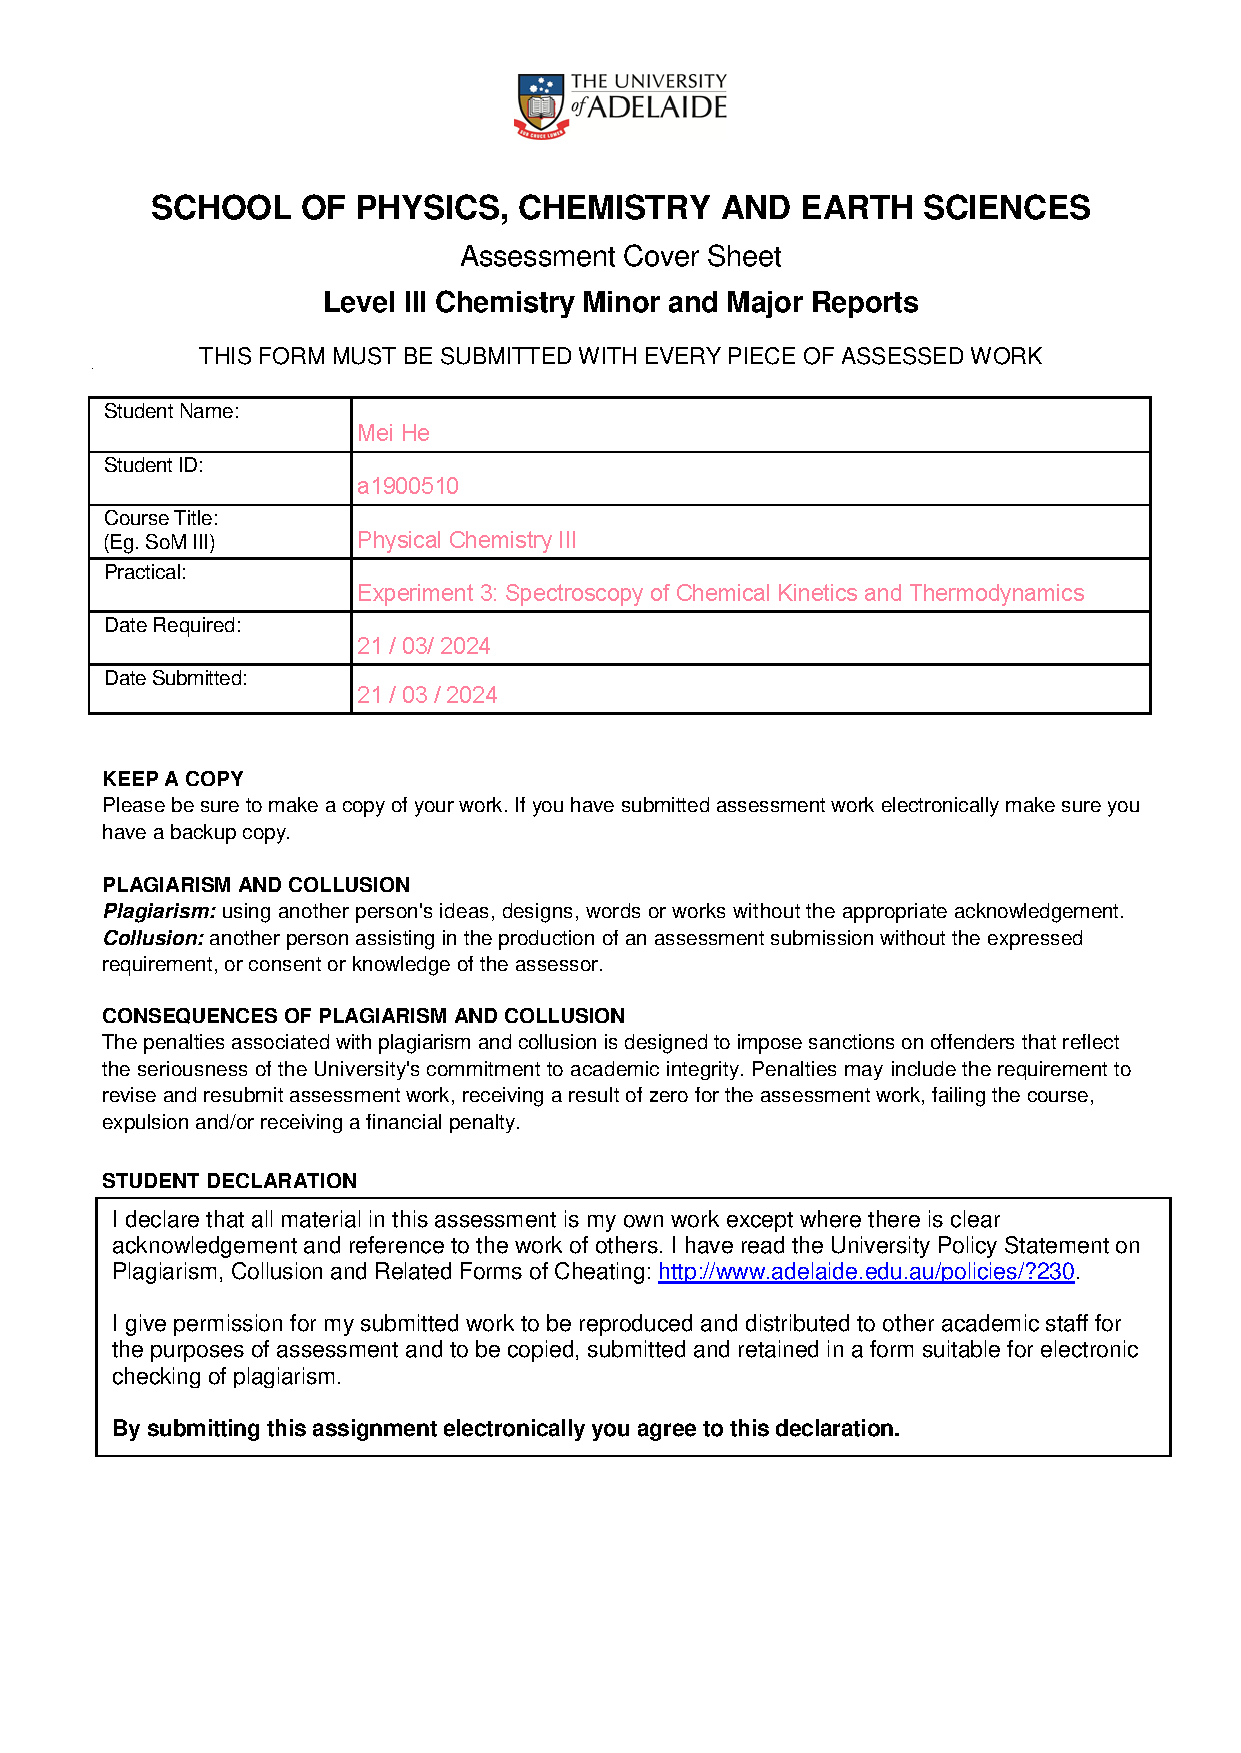
\includepdf[pages=-]{exp3_cover.pdf}


%%%%%%%%%%%%%%%%%%%%%%%%%%%%%%555
% title page
\begin{titlepage}
  \centering
  
  {\LARGE \titlestr \par}

  \vspace{1cm}
  {\Large \authorstr \par}

  {\bf A1900510}

  \vspace{1cm}
Thursday March 7 2024     % PUT YOUR DATE HERE

  \vspace{1cm}
  Report submitted for
  {\bf Physical Chemistry III}
  at the University of Adelaide. \textbf{Due 23:59pm March 21st 2024}

  \vspace{1cm}
    \begin{abstract}
        chuck abstract here
    \end{abstract}
  \vspace{1cm}
  \tableofcontents
  \listoffigures

  \vfill
\end{titlepage}

% put headings on each page
\pagestyle{fancy}
\fancyhf{}
\rhead{\shorttitlestr}
\lhead{\authorstr}
\rfoot{Page \thepage\ of \pageref{lastcontentpage}}
\renewcommand{\headrulewidth}{1pt}

%%%%%%%%%%%%%%%%%%%%%%%%%%%%%%555
% main report
\clearpage


%%%%%%%%%%%%%%%%%%%%%%%%%%%%%%555
% intro
\section{Introduction}
A short introductory section incorporating the experimental aims. You may include figures and diagrams, but
these should be prepared yourself or properly attributed.


- first part uses emission spectroscopy to measure rate of electron transfer from phoot excited transition metal complex to another species. In this case, the competition between light emissio  and electron transfer enabkes a sensitive measurement of the electron transfer rate, given knowledge of je rate of relaxation of tje excited state in the absence of the electron transfer partner

in second aprt, use absorption spectrophotomeyry to determine the empirical formula ajdn equilibrium stability constant of a transition metal complex based on changes to hte absorption spectrum as a function of hte concentrations of te chemical components of the complex that are mixed together

aims: top use spectroscopy nad spectrophotometry to measure rxn rate coefficients and equilibrium constants of physiochemcial processes
- understand relationship between absorption., emission and excitation specra of a molecule
understand what a stern-volmer plit is and hw it can be used to measure rxn rate coefficients from measurements of luminescence quenching
distinguish between diffusion limited and rxn limited processes

isosbestic point n figure ut whsat it means
\textbf{from here is legit}
The experiment consisted of two parts in order to investigate the kinetics and thermodynamics of chemical processes, using spectroscopy and spectophotometry.

In the presence of a quenching species, luminescent molecules 

The Franck-Condon principle states that the vertical transition to occur when the absorption of light results in an electronic excited state with the same spin multiplicity \autocite{frank_condon}.

Part 1 investigated the electron transfer rate from luminescent quenching of \ce{Ru(bpy)_{3}^{2+}} by \ce{Fe^{3+} and \ce{Cu^{2+}}}. As per the lab manual\autocite{lab_manual}, the excited state of a luminescent molecule can be deactivated by the presence of a quencher molecule which inhibits emission of light. The absorption of light 


half page, 3-5 paras, talk about absorption vs excitation vs emission, go into frank condon principle, quenching, electron transfer and rate (put figs)
A short introductory section incorporating the experimental aims. You may include figures and diagrams, but
these should be prepared yourself or properly attributed.
%%%%%%%%%%%%%%%%%%%%%%%%%%%%%%555
% experiment
\section{Experiment}
An experimental section. The experimental section will have a more experiment specific component but adequate 
details of what was done in the practical still need to be provided

\documentclass[main.tex]{subfiles}
\graphicspath{{\subfix{../images/}}}
\begin{document}

As per the lab manual.
\autocite{lab_manual}



\end{document}



%%%%%%%%%%%%%%%%%%%%%%%%%%%%%%555
% Results
\section{Results \& Discussion}


LEAVING AS EXAMPLE
Thus, the equation for the calibration curve is:
\begin{equation*}
    \mathcolorbox{Lavender}{A = 0.21066718C_{\text{digested}} -0.0077607}
\end{equation*}

A results and discussion section which integrates answers to the questions above, assignment of spectra, 
includes a discussion of yields and data collected. It is useful if you include subheadings etc to draw attention to 
the answers you provide to the questions.

As large volumes of data are generated or extensive calculations will be done, the results of these need 
to be presented in an appropriate style (graph, table or figure) and these results need to be described 
and discussed in the context of the experimental aims.

\subsection{Electron Transfer Kinetics via Emission Spectroscopy}
\subsubsection*{Results}
\begin{figure}[H]
    \centering
    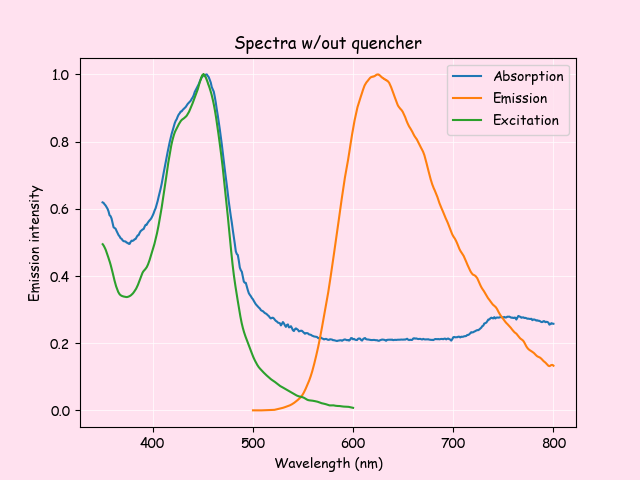
\includegraphics[width = 0.7\linewidth]{part1_noq.png}
    \caption{REDO TITLE}
    \label{fig:enter-label}
\end{figure}
\subsubsection*{In Class Analysis}
\textbf{Question 1} 
\begin{figure}[H]
     \centering
     \begin{subfigure}[b]{0.49\textwidth}
         \centering
         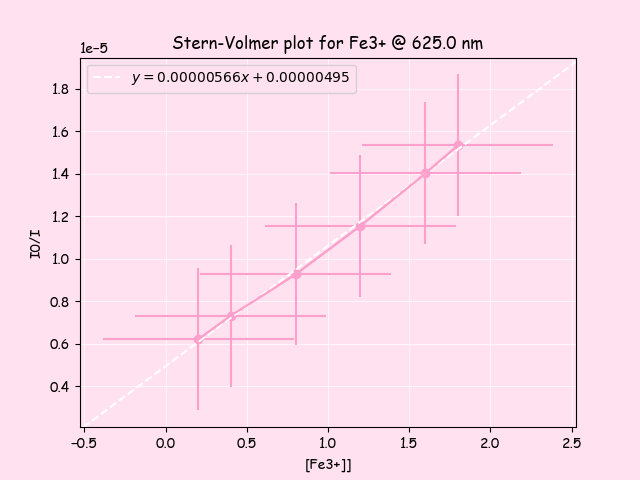
\includegraphics[width=\textwidth]{part1_q1_Fe.png}
         \caption{\ce{Fe^{3+}}}
         \label{fig:part1_q1_fe}
     \end{subfigure}
     \hfill
     \begin{subfigure}[b]{0.49\textwidth}
         \centering
         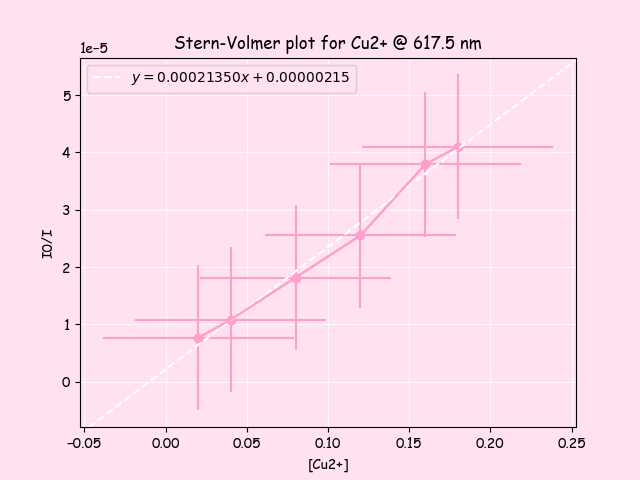
\includegraphics[width=\textwidth]{part1_q1_Cu.png}
         \caption{\ce{Cu^{2+}}}
         \label{fig:part1_q1_Cu}
     \end{subfigure}
     \caption{Stern-Volmer plots for luminescent quenching measurements}
     \label{fig:stern_volmers}
\end{figure}

Figure \ref{fig:stern_volmers} represents the following curve (eqn (6)) from lab manual\autocite{lab_manual}:
\begin{equation*}
    \frac{I_0}{I} = 1 + \frac{k_q}{k_d}[Q]
\end{equation*}

So $\frac{k_q}{k_d}$ is the slope of each curve. So:
\begin{equation*}
    \mathcolorbox{Lavender}{\frac{dy}{dx}_{\text{Fe}^{3+}} = \input{part1_q1_fe_slope.txt} \text{ @ } \input{part1_q1_fe_wl.txt} \text{ nm} }
\end{equation*}
And
\begin{equation*}
    \mathcolorbox{Lavender}{\frac{dy}{dx}_{\text{Cu}^{2+}} = \input{part1_q1_cu_slope.txt} \text{ @ } \input{part1_q1_cu_wl.txt} \text{ nm} }
\end{equation*}
\\
\textbf{Question 2}
\par From the lab manual\autocite{lab_manual}, $k_d = 1.7 \times 10^6\text {s}^{-1}$. Thus,
\begin{equation}
    k_q = \text{slope} \times k_d
    \label{eq:p1q2}
\end{equation}
Substituting slopes to equation (\ref{eq:p1q2}):
\begin{equation*}
    \mathcolorbox{Lavender}{k_{q,\text{Fe}^{3+}} = \input{part1_q2_fe.txt} \text{ s}^{-1}}
\end{equation*}
\begin{equation*}
    \mathcolorbox{Lavender}{k_{q,\text{Cu}^{2+}} = \input{part1_q2_cu.txt} \text{ s}^{-1}}
\end{equation*}
\\
\textbf{Question 3}
\par From tables 2 and 3 in the lab manual\autocite{lab_manual}:
   $ k_{11} = 1 \times 10 ^ 8 \text{ M}^{-1}\text{s}^{-1}$, 
    $k_{22, \text{Fe}^{3+}} = 4 \text{ M}^{-1}\text{s}^{-1}$, 
    $k_{22, \text{Cu}^{2+}} = 1 \times 10 ^ {-5} \text{ M}^{-1}\text{s}^{-1}$. And standard reduction potentials: $E^{\circ}_{\text{R}^{3+}} = -0.8 \text{ V}$, $E^{\circ}_{\text{Fe}^{3+}} = 0.77 \text{ V}$, $E^{\circ}_{\text{Cu}^{2+}} = 0.16 \text{ V}$.
\\ Since $E^{\circ}_{\text{Cell}} = E^{\circ}_{\text{Red}} + E^{\circ}_{\text{Ox}}$, 
\begin{equation}
    E^{\circ}_{\text{Cell}} = E^{\circ}_{\text{Red}} + 0.8 \text{ V}
    \label{eq:ecell}
\end{equation}
Rearranging equations (13) and (12) respectively from the lab manual\autocite{lab_manual},
\begin{equation}
    K_{12} = e^{\frac{zF}{RT}E^{\circ}_{\text{Cell}}}
    \label{eq:K12}
\end{equation}
\begin{equation}
    f_{12} = e^{\frac{(\ln{K_{12}})^2}{4\ln{(k_{11}k_{22} / Z_{12}^2)}}}
    \label{eq:f12}
\end{equation}
Equation (11) from the lab manual\autocite{lab_manual} gives:
\begin{equation}
    k_{\text{ET}} = k_{12} \approx \sqrt{k_{11}k_{22}K_{12}f_{12}}
    \label{eq:ket}
\end{equation}
Where $Z_{12} \approx 10^{11} \text{ M}^{-1} \text{s}^{-1}$, $T = 298.15\text{ K}$, and $F = 96485.3399 \text{ Cmol}^{-1}$.
\\
\par The below Python function (see Appendix \ref{appx:part1_code} for full script) takes inputs for ($k_{22}$, $E^{\circ}_{\text{Red}}$, $z$), and substitutes above given values, equations (\ref{eq:ecell}), (\ref{eq:K12}), and (\ref{eq:f12}) to equation (\ref{eq:ket}), to return the $k_{\text{ET}}$ value.
\input{marcus_theory_fn.txt}
This function was called for ($k_{22 \text{Fe}^{3+}}$, $E^{\circ}_{\text{Fe}^{3+}}$, $z = 3$), and ($k_{22, \text{Cu}^{2+}}$, $E^{\circ}_{\text{Cu}^{2+}}$, $z = 2$) to respectively return
\begin{equation*}
    \mathcolorbox{Lavender}{k_{\text{ET},\text{Fe}^{3+}} = \input{part1_q3_fe.txt} \text{ M}^{-1} \text{s}^{-1}}
\end{equation*}
\begin{equation*}
    \mathcolorbox{Lavender}{k_{\text{ET},\text{Cu}^{2+}} = \input{part1_q3_cu.txt} \text{ M}^{-1} \text{s}^{-1}}
\end{equation*}

\subsubsection*{Discussion Questions}

\subsection{Part 2}







% concl
\section{Conclusion}
\documentclass[main.tex]{subfiles}
\graphicspath{{\subfix{../images/}}}
\begin{document}

Using UV-Vis spectrometry to analyse digested iron tablet samples, the mass of iron in three tests of were found to be 97.1922855mg (88.3112496 - 107.05773mg), 89.8571711mg (81.3420968 - 99.316089mg), and 92.8664488mg (84.2012364 - 102.492147mg). Which support the manufacturer's claim of 87.4


\end{document}
\label{lastcontentpage}

%%%%%%%%%%%%%%%%%%%%%%%%%%%%%%555
% references
\addcontentsline{toc}{section}{References}

\printbibliography

\newpage
\appendixpagenumbering
\begin{appendices}
\subsection{Part 1}
\label{appx:part1_code}
\input{part1.txt}

\subsection{Part 2}
\label{appx:part2_code}
\input{part2.txt}
\end{appendices}
\end{document}


 